\documentclass[a4paper,12pt]{article}
\usepackage[margin=2.5cm]{geometry}
\usepackage{setspace}
\onehalfspacing

\usepackage{array}
\usepackage{multirow}
\usepackage{csquotes}
\usepackage[usenames,dvipsnames]{color}
\usepackage[utf8]{inputenc}
\usepackage{pdfpages}
\usepackage{rotating}
\usepackage{longtable}
\usepackage[labelfont=it]{caption}
\usepackage{color}
\usepackage{soul}

\usepackage{titling}
\newcommand{\subtitle}[1]{%
  \posttitle{%
    \par\end{center}
    \begin{center}\large#1\end{center}
    \vskip0.5em}%
}

% Highlight
\definecolor{highlightyellow}{rgb}{1,1,0.7}
\sethlcolor{highlightyellow}
\makeatletter
\newcommand\fix{%
  \let\set@color\beamerorig@set@color
  \let\reset@color\beamerorig@reset@color}
\makeatother

% Note and Source below tables and figures
\usepackage{threeparttable}% Alternative for Notes below table
\newcommand{\Figtext}[1]{%
	\begin{tablenotes}[para,flushleft]
		\hangindent=1em
		\footnotesize
		\raggedright
		#1
	\end{tablenotes}
}
\newcommand{\Fignote}[1]{\Figtext{\emph{Note:~}~#1}}
\newcommand{\Figsource}[1]{\Figtext{\emph{Source:~}~#1}}

% TITLE PAGE
\title{\Large {\bf Auction or haggling -- what should the seller choose?} \\ A look at the interaction between price discovery and competition in Name-Your-Own-Price auctions.}
\subtitle{(First draft)}
\author{Jonas K. Sekamane}
\date{28. November 2014\thanks{This paper is written for the seminar \emph{Experiments in Economics} at the Department of Economics, Universisty of Copenhagen in the autum 2014. Supervison by Ulrik Haagen Nielsen.}}

% NEW COMMANDS AND TYPES
\newcolumntype{x}[1]{%
>{\raggedright\hspace{0pt}}p{#1}}%


\begin{document}
	
	\pagenumbering{gobble}% Remove page numbers
	\clearpage
	\thispagestyle{empty}
	
	\maketitle{}
		
	\newpage
	
	\clearpage %  Reset page numbers to 1
	\pagenumbering{arabic}
	\setcounter{page}{1}
	
	\begin{abstract}
		{...}
	\end{abstract}
	
	\tableofcontents
	
	\newpage

	\section{Introduction}

	Which price mechanism should the seller choose? This article focuses on the selling of unique objects or scarce goods, i.e. where multiple buyers compete for the same object. This has traditionally been the realm of auctions (art, antiques, collectibles, etc). But perhaps -- and contrary to popular believe -- the standard single-item auction formats are not the optimal selling methods. An alternative price mechanism is Name-Your-Own-Price (NYOP). In NYOP the buyer proposes a price. If the proposed price is above some threshold level, that is set by the seller, then the buyer gets the object at the proposed price. A previous experiment by Shapiro and Zillante (2009) shows that NYOP gives sellers higher revenue than a simple posted price mechanism. The experiment in this paper tries to answer; if using a NYOP also gives higher revenue than an english auction? To answer this one has to introduce competition into the NYOP. The natural follow-up question is then why. Why revenue is higher in NYOP, or why revenue is not higher? To try and answer the latter two questions, additional NYOP treatments are proposed. These treatments focus on the interaction between price discovery and competition, and how these affect the results.

	This paper is structured as follows. First the various prices mechanisms (posted price, NYOP, haggling, english auction and buyout auction) are introduced. This section also includes a discussion of how the various price mechanisms relate to one another. This is followed by a short summary of the literature, previous experimental findings and some theoretical predictions. Hereafter follows the full description of the experiment; its design, treatments, recruitment, participant requirements and the technical implementation. The last sections of this paper includes a recapitulation of hypotheses and expected results from the experiment, the shortcomings of the experiment, future extensions, and the conclusion.

	\section{Various price mechanisms}

	\subsection{Posted Price}
	The simplest and most common price mechanism is a posted price (also known as {\it listed price}, or {\it take-it-or-leave-it offer}). You encounter this price mechanism everyday when going to the supermarket or a retail shop. Here the seller proposes and sets the price. The price is visible to all, and buyers can only choose to buy the item at the posted price, or choose not to buy. The item is (usually) sold to the first buyer willing to make the purchase. There is often no official count down or time limit on the offer. However, 1) if only a single and unique item is put up of for sale, then the first-come-first-served (FCFS) allocation rule imposes a sort of time pressure on competing buyers to swiftly make their purchasing decision. (If multiple items are put up for sale, and buyers desire at most one item each, then competition would be less fierce and the time pressure weaker). 2) Occasionally assortments change and unsold items are removed\footnote{\label{footnote:price_reduction}Often one or several price reductions are attempted before an unsold item is removed, but these dynamics are beyond the scope of this paper.}. While the individual seller might prefer no time limit, consumer-to-consumer marketplaces like DBA.dk impose a limit. One motivation for this is undoubtedly that the marketplace tries to balance the buyers' signal-to-noise ratio in terms of desirable items when buyers browse through the marketplace. A time limit is a simple measure restricting the accumulation of unsold and hence undesirable items. Besides the simplicity, familiarity and generality of the posted price mechanism, a main advantage is that the seller has full control over the final price. If sellers are risk averse this may be the decisive feature when picking a price mechanism. A disadvantage for sellers is the unspecific transfer date, especially if the there are costs associated with storing the item or if the item is perishable. This of course ties into an other main disadvantage -- the lack of a price discovery process. What is the optimal posted price that the seller should set? If the seller sets the price too low the item is sold very quickly, and if its set too high, the item is sold slowly or not at all. Often the seller will be uncertain about the value of the item, perhaps not the seller's own valuation or reserve price, but uncertain about what the the highest value is among all potential buyers. This problem is even more prevalent when selling a single and unique item. Because there is often no prior market price to guide the seller, and because individual buyers may value the uniqueness and exclusivity, far beyond the mere production costs of the item.

	\subsection{Name-your-own-price (NYOP)}

	The name-your-own-price mechanism (also known as {\it reverse pricing} or {\it name-your-own-price auction}) is an extension of the posted price mechanism. The seller decides the posted price and a threshold level at which he or she is willing to sell the item. The threshold level bears some similarities with a reserve price in auctions and a price reduction in the posted price mechanism (see footnote \ref{footnote:price_reduction}). Only the posted price and the buyer's own value is known to the buyer, who now have one additional option besides `buy', and `don't buy'. The buyers can submit a bid. Their bid is rejected if it is below the threshold level. And if above, the bid is accepted and the transaction is made with the buyer. This is the essential parts of the NYOP mechanism, but there exist numerous extensions and modifications. Before I discuss these I would like to briefly present one striking result of the NYOP.

	Shapiro and Zillante (2009) finds that revenue is higher when using the NYOP mechanism instead of using a posted price mechanism. One might intuitively expect that revenue was lower since buyers that could afford the posted price, would instead use the NYOP option, and get the item cheaper. But what drives their results is 1) new buyers that could not afford the item at the posted price, and 2) buyers with values much higher than the posted price, that still use the `buy' option and pay the posted price. The latter also puzzles the two authors, since submitting a bid is a dominant strategy. It is dominant because buyers can choose the to `buy' after their bid has been rejected in their particular NYOP setup. Their explanation is that there is some non-monetary mental cost or haggling cost associated with bidding (clicking more buttons, disutility of rejected bid, etc), that the buyers avoid if they just use the `buy' option.

	Thus there is a whole branch of modifications in the options presented to buyers after their bid has been rejected. One modification is to remove the `buy' option from the buyers initial set of choices. Such that the buyer can only `bid' or `don't buy', and only if the bid is rejected can the buyer `buy' the item at the posted price. Shapiro and Zillante (2009) show that this modification also gives the seller a higher revenue than the posted price, but the increase in revenue is not as large. Another modification they try is hiding the posted price, but having less cues about the threshold level reduces the average bid. Clearly presenting the posted price has a sort of anchoring effect\footnote{In the behavioural economics literature the `anchor' generally does not add any relevant information to the agents decision -- yet the irrelevant `anchor' still affects the outcome of the decision. In NYOP the posted price contains relevant information about the threshold level.} or reference price. Yet another modification is the `opaque feature'. Here the buyer is uncertain about the exact properties of the product purchased (e.g. the buyer knows that it is a three-star hotel in New York, but not which hotel). It will not discuss this in more detail, but just note that Shapiro and Zillante hypothesis that the fear of buyers learning the threshold level might be the reason why marketplaces have an opaque feature (emphasis added):
	\blockquote[Shapiro and Zillante, 2009, p.737]{\emph{ ... Priceline customers are more likely to purchase the same product many times (e.g. a ticket between New York City and Los Angeles) and consequently there is a substantial \emph{\bf risk that customers might quickly learn the threshold range and decrease their bids}. When this is not the case, as at http://www.prisminister.dk which sells consumer electronics, the NYOP website does not have the opaque feature. Indeed, it is simply \emph{\bf less likely that one person would be buying a washer repeatedly and consequently the customer's information about the threshold is less precise} ...}}

	The NYOP mechanism has mostly been studied as a method to curb excess capacity/supply. On the internet Priceline.com has been the pioneer of the NYOP mechanism, selling excess hotel capacity and excess seats on planes (Shapiro and Zillante, 2009). Consequently the literature on NYOP assumes that there are items enough for every buyer willing to purchase. There is no constraint on the supply of items for sale and hence no competition among buyers for the items unlike auctions (Shapiro, 2011). In latter sections I will try to introduce competition in the NYOP and study learning through repeated bidding. To my knowledge no prior paper has incorporated competition into the NYOP nor explicitly studied learning in NYOP.

	\begin{figure}
	        \centering
	        \caption{NYOP game tree}
	        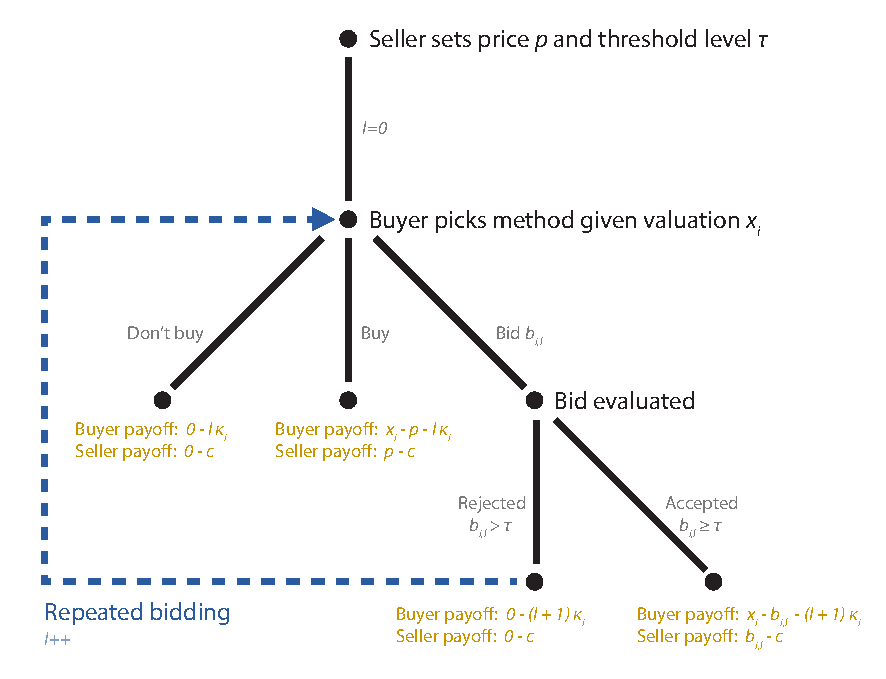
\includegraphics[width=\textwidth]{Figures/NYOP_GameTree}
			\label{fig:game_tree}
			\Fignote{Note: Where $l$ is number of bids attempted, $\kappa_i$ is haggling cost of buyer $i$, $c$ is marginal cost, $\tau$ is threshold level, $p$ is posted price, $x_i$ is value of buyer $i$ and where $b_{i,l}$ is the $l$'th bid of buyer $i$.}
	\end{figure}

	The NYOP could be further extended by allowing repeated bidding, see figure~\ref{fig:game_tree}. If a bid is reject the buyer can `buy', `don't buy' or `bid' a higher amount. In addition it is normal to assume that buyers endure some non-monetary mental cost or haggling cost from bidding (clicking more buttons, disutility of rejected bid, etc). As Terwiesch et. al. (2005) note this implies that buyers will be balancing between bidding too much, giving the seller additional rents, and bidding too little, possibly enduring further haggling cost. Or worse, in the case of not winning the item, wasting haggling cost. With significant haggling cost, the seller would (indirectly) price discriminates buyers based on their haggling cost. Buyers that are more willing to haggle (lower haggling cost) can archive lower prices and higher payoffs. Terwiesch et. al. (2005) argue that fairness concerns as well as legal constraints prohibit more systematic price discrimination. The seller cannot price discriminate on other parameters. E.g. the seller cannot change the threshold level based on the identity of the buyer, nor change the threshold based on the bidding sequence. Buyers purchasing an item at the same point in time must be charged the same price.

	One advantage of the NYOP is that seller maintains control over the final price. The lowest possible final price will be the threshold level. The other advantage is that the NYOP has a built-in price discovery process. Buyers with values below the posted price, but above the seller's threshold level might purchase an item. The seller's uncertainty about the value, is less critical since they don't need to select an optimal price point, but select an optimal price range.

	\subsection{Haggling}

	As previously hinted at, the NYOP mechanism is not far from haggling or models of {\it bargaining}. In bargaining 1) agents can enter a mutually beneficial agreement, 2) there is a conflict of interest over the agreement and 3) an agreement cannot be reached without the approval of all agents (Terwiesch et. al., 2005). Bargaining can been formulated as a procedure where agents sequentially make decisions. A distinct difference between haggling and repeated-bidding NYOP is that the seller does not initially set or commit to a threshold level. Instead the seller evaluates each bid as they tick in. Hence the threshold variable $\tau$ is not necessarily constant, but could be a function of the buyer identity $i$, the number of attempted bids $l$, the sellers impatience, and the set of previously submitted bids by other buyers $b_{j,l}$. Often, even in simple bargaining models, multiple equilibria arise.

	The NYOP haggling model proposed by Terwiesch et. al. (2005) assumes that the threshold level is constant. Furthermore it assumes that all uncertainties (other buyers' value, other buyers' beliefs, etc) can be lumped together into a single distribution. This way the problem of finding equilibrium simplifies to a problem of search. In this search problem buyers balance between search efforts (by minimising haggling costs or bids) and choosing a bid that is just above the threshold level (by bidding repeatedly and incrementally until a bid is accepted). A key requirement, that allows sellers to charge a price above the marginal cost, is that haggling costs are non-zero.

	\subsection{English auction}

	In standard auctions the buyer with the highest bids wins the item. In the first-price auction the winner pays his own (highest) bid. In second-price auctions the transaction price is the second highest bid. In the latter the buyer does not shade his or her bid, but in theory bids his or her true value. In both cases each buyer submits a single bid and the bids are sealed. In the english auction bids are open and visible to all. Buyers continue to incrementally outbid each other until there is no challenger, or until the clock runs out. The linkage principle tells us that revenue in the english auction is as least as large as in the second-price auction (Krishna, 2009). There are good theoretical results ranking the revenue of most standard auction formats. And many experimental studies have been carried out trying to confirm these results (Kagel and Levin, 2011). 

	{\bf Reserve prices.} Normally bidding starts at zero, however the seller may set a reserve price or starting bid. The seller should set the reserve price such that it exceeds his or her value, since the reserve price becomes the minimum revenue that the seller will receive. Bidding starts at the reserve price, and buyers cannot bid below this. In theory a reserve price can increase the revenue of sellers, since it can extract addition surplus from the highest bidder (Haruvy and Leszczyc, 2010)\footnote{This is conditional on the item being sold. If the reserve price is set too high, such that the item is no longer sold, the reserve price may reduce revenue. This may happen when the exclusion principle no longer holds (Krishna, 2009).}. Empirical evidence question this theoretical result. The reserve price implies fewer participants in the auction, which may in turn lead to lower prices and revenue. This could happen because of competing auctions where participants choose the auction with the lowest reserve or with no reserve price (Haruvy and Leszczyc, 2010). An alternative explanation is that fewer participants, leads to less competitive arousal or less `frenzy' and that this is what gives lower prices and revenue (more on the latter below when the discovery process is discussed). The reserve price is visible to all. 

	Alternatively sellers can use a secret reserve price, where buyers only know that a reserve price exists, but not its value. Thus when bidding they form prior expectations about the value of the reserve price. When the auction ends the buyer with the highest bid wins, but only if the bid is above the secret reserve price. Unlike the reserve price, the secret reserve price should not lead to fewer participants in the auction. This has been disputed and the empirical evidence on secret reserve price and revenue is not unanimous (Haruvy and Leszczyc, 2010). I mention the reserves price here, since they bear some similarities with the threshold level in the NYOP auction.

	{\bf Buyout auctions} or {\it buy-it-now} price is other modification to auctions that bears similarities with the NYOP mechanism. The buyout option has been popularised by internet marketplaces such as eBay. Besides bidding in the auction as describe above, buyers have the option to purchase the item at the posted price ending the auction before the clock runs out (temporary {\it buy-it-now} option can also be found on eBay, here the {\it buy-it-now} option disappears once the auction receives its first bid). Buyers will choose the buy-it-now option if their time-sensitivity, transaction costs or disutility from not winning the auction is sufficiently large (Haruvy and Leszczyc, 2010). The {\it buy-it-now} price has puzzled researchers since it places a maximum on the expected revenue of the seller. One possible explanation is that, when buyers are risk averse, a carefully selected price under {\it buy-it-now} may increase revenue. It does so by extracting the risk premium buyers are willing to pay to avoid losing the auction (Kagel and Levin, 2011).
%\fix\hl{*** Look more at explanations from buy-it-now literature, since it may also hold the key/answers to why/why not NYOP would outperform Auction ***}

	{\bf Duration} of the auction is another important parameter, especially in internet auctions that can stretch over several days. In long-duration auctions the individual buyer takes his or her time-sensitivity or impatience into account when bidding. Secondly, the duration of the auction will affect the discovery process of the auction. If one imagines that the process by which buyers discover the auction is random, then the longer the duration, the more buyers will find and participate in the auction, which should lead to higher revenue. Haruvy and Leszczyc (2010) summaries a field experiment conducted on eBay and at a local auction platform. The experiment finds that on eBay a longer duration results in higher revenue, while the opposite is true at the local auction and both relations are significant. Haruvy and Leszczyc (2010) argue that this is due to the random arrival process at eBay auctions, while the local auction attracts buyers in higher concentrations, by sending out invitations. Therefore longer duration at the local auction does not lead to more participants, but just less competitive arousal and lower revenue. 

This finding touches on when and why a posted price mechanism or a NYOP mechanism might be preferable to a auction. If the arrival time of buyers is long, then a auction with a short time frame is unattractive because of few participating bidders. Empirically evidence show that the expected revenue in auctions decrease as the number of buyers decrease (SOURCE). But an auction with too long a time frame might equally well be unattractive, if it fore instances lowers the competitive arousal of buyers, leading to lower bids or less out-bidding. The seller can set the optimal duration of the auction, but in most cases is seems unlikely that the seller can significantly influence the arrival process of buyers. And hence there may be arrival process (like long arrival times of buyers) where a posted price mechanism or NYOP mechanism is preferable to auctions. Since competition among buyers in these two mechanism rely less buyers interacting simultaneously.

	{\bf Snipping behaviour.} Auctions with `hard close' (a fixed, announced end time) often see snipping behaviour. Buyers simply wait until the very last minutes or seconds before they submit bids. The rationale is that by submitting last-minute bids the buyer does not reveal information to other buyers. Often it will be a small subset of knowledgeable buyers that engage in sniping. Having a `soft close' ending (where bids receive shortly before the end time extends the duration of the auction) is one way in which snipping behaviour can be avoided. Another option is a \emph{candle auction} were the end time is unknown to buyers. % Implementing a proxy bidding system, where buyers can submit a sealed max-bid is another way to discourage sniping behaviour. A computer then automatically out-bids others, until the max-bid is reached.

	Auctions have many advantages. One is the price discovery process, that may lead to higher expected profits that the posted price mechanism. This is an especially appealing feature when selling scarce goods where the seller is uncertain about the value. Another advantage is that standard auctions are efficient since they allocate the item to the buyer with the highest value (see \ref{footnote:efficient}). Another advantage over the posted price, is that auctions have more or less fixed durations, and the seller is almost certain to get the item off his or her hands. A disadvantage is that the seller has no control over the final price. This may especially be problematic for risk averse sellers. Some solutions to this has been discussed above, such as reserve price or secret reserve price.

	I choose the english auction, firstly because this format has the most features in common with the NYOP, hence it is easier to interpret the results as {\it ceteris paribus}. Secondly, because it has an element of learning and competition build in, which is the main focus of the NYOP treatments. Learning happens in the english auction since bidders can bid repeatedly and see the bids of other buyers. Competition is present in all auctions, because of scarce supply and an allocation rule that says the highest bidder wins the item. Since I am not interested in studying the snipping behaviour of a subset of buyers, but rather learning and group learning, the experiment will use randomly varying duration also known as a {\it candle auction}.

	\section{Literature review}

This section will review some of the theoretical and experimental results in the literature. The main focus will be on explaining the difference in revenue between the posted price, NYOP, and auction mechanism. And some focus will also be given to learning and competition in the NYOP.

%	| Article                           | Mechanism              | Object    | Bidding   | Comments |
%	| -------------                     |:------------- :       | :-----    | :----     | :-----  |
%	| Shapiro and Zillante (2009)       | NYOP, Posted-price    | multiple (no competition)  | single-bid | ... |

	{\bf Posted price vs auctions}
%	> … finding the optimal posted price involves product-category expertise as well as demand and competition research … category expertise is more useful for posted pricing, experienced sellers specializing in a product category should use posted prices more than auction.  

	{\bf Posted price vs NYOP}


	\section{Experiment}

	Why use an experiment to investigate auctions and the NYOP mechanism? Wouldn't it be equally or more fruitful to set up models and solve them analytically? There are two main problems with the analytical approach, that one avoids with an empirical or experimental approach. First, the analytical solution often lead to multiple equilibrium or is intractable due to the complexity of the model (see earlier discussion on bargaining models). Secondly, the actual characteristics of buyers and hence their behaviour is vastly unknown. The literature has well established concepts such as `risk aversion' or `anchoring effect' -- but whether, why or when buyers are risk averse remains a mystery in most settings. Haruvy and Leszczyc touch upon these issues in their discussion of traditional auctions vs online auctions:
	\blockquote[Haruvy and Leszczyc, 2010 pp.61-62]{\emph{Traditional auction theory builds heavily on bidder rationality, in many cases risk neutrality, bidder symmetry, revenue and strategic equivalences, and other key properties that are … known to be violated in traditional auction settings as well … In our opinion, based on the research reviewed here, questions of optimal design choice in online auctions can often be addressed empirically and have as much to do with bidder preferences, bidder search, mental processing of information, and issues of trust and reputation as they do with the traditional focus on equilibrium predictions. }}


	\subsection{Design}

	To explain the resulting difference between auctions and NYOP, I will compare the NYOP results to three alternative NYOP treatments. My hypothesis is that in particular two counteracting factors effects the results of the NYOP mechanism:

	\begin{enumerate}
		\item {\bf Learning} or price discovery. Through experience and information about previously submitted bids buyers will learn and come to form correct expectations about the seller's threshold level. This will, everything else equal, result in buyers submitting bids closer to the threshold and significantly below the posted price, thus having a negative effect on the seller's expected revenue. Learning happens through three different channels; 1) the \emph{individual channel} where buyers bid repeatedly and incrementally until they reach the threshold level, 2) the \emph{common channel} where buyers observe what others bid and use this to form expectations about the threshold level, and 3) the \emph{experience channel} where buyers participating in multiple rounds, learn the winning bids in each round, and use this to form expectations about the general distribution of the threshold level.
	 	\item {\bf Competition}. When there are fewer items for sale, it pressures buyers into submitting earlier bids under the NYOP, since the first bid above the threshold level wins the item. The allocation rule in the NYOP is henceforward referred to as First-Come-First-Served (FCFS). The pressure to submit an early bid will, everything else equal, imply that buyers have less time available to discover the threshold level. And hence buyers will to a lesser extend try to shade their bids, or alternatively not engage in bid-shading but simply use the `buy' option. This will have a positive effect on the seller's expected revenue\footnote{Competition likewise exists in auctions formats, since here the allocation rule determines that the buyer with the highest (HIGH) bid wins the auction.}. As earlier noted Shapiro and Zillante (2009) found that an important factor increasing revenue in the NYOP, was the participation of new buyer that were not able to purchase at the posted price. Whether fewer objects lead to higher revenue, will likewise depend on the fraction of new buyers that manage to acquire the item.
	\end{enumerate}

	Participants in the experiments will all play the role of buyers. This experiment is interested in studying the behaviour of buyers under different mechanisms. To simplify and control for the behaviour of the seller, the actions of the seller is carried out by a computer. The seller chooses a posted price and threshold level. Each session will have 5 participants ($N=5$).

	In each round, $t$, the values of buyers, the seller's posted price and threshold level are all randomly drawn from uniform distributions, similar to Shapiro and Zillante (2009). In each period the buyers' values are drawn from $U(a_t , a_t + 400)$, where $a_t$ is drawn in each round from $U(0, 1600)$. The lowest value distribution in any round thereby becomes $U(0, 400)$ and the highest $U(1600, 2000)$ and overall values can range between 0 and 2000. Buyers only see their own value and the posted price, they don't receive any information on the distributions. The posted price is the midpoint of the value distribution $p_t = a_t + 200$, and the seller's marginal cost is $a_t$. Hence the posted price is the monopoly price. The threshold level is drawn from $U(a_t, p_t)$. See figure~\ref{fig:distribution}. In the english auction only the buyers' values and posted price is used. There is no reserve price or secret reserve price, but bids have to be strictly positive.
	
	\begin{figure}[h]
	        \centering
	        \caption{Overview of values and distributions}
	        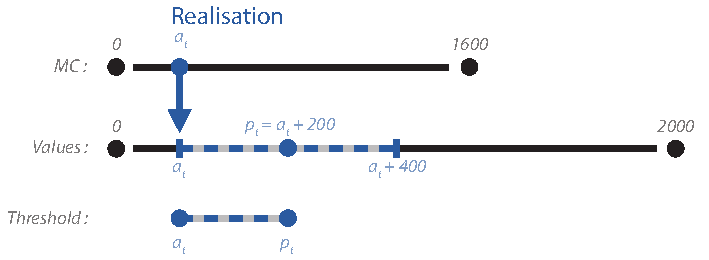
\includegraphics[width=0.7\textwidth]{Figures/Distribution}
			\label{fig:distribution}
	\end{figure}

	Each session has 5 treatments, and 8 rounds per treatment. So each participant goes through a total of 40 rounds. 8 rounds should be enough to uncover learning through the experience channel, and not too long, such that it demotivates participants. The duration of each round (in seconds) is drawn randomly from the uniform distribution $U(60, 120)$. Participants will be told that the duration varies, and told that ``each rounds may last a couple of minutes'', but otherwise not be given any information about the distribution and there is no visible countdown. As mention earlier this is done to avoid snipping and encourage early bidding in the auction. The NYOP treatments may end before the clock runs out, if all items have been sold. The order of treatments will vary with session. By varying order one can afterwards test and ensure that the results are not due to a particular ordering (known as spill-over effects). The auction treatment is either first or last, since different instructions are needed, and to give participants an experience of continuum. Sessions will use one of the following five orderings:

\[	{AUCTION_0, NYOP_0, NYOP_P, NYOP_S, NYOP_M} \]
\[	{AUCTION_0, NYOP_M, NYOP_S, NYOP_P, NYOP_0} \]
\[	{AUCTION_0, NYOP_P, NYOP_M, NYOP_0, NYOP_S} \]
\[	{NYOP_M, NYOP_P, NYOP_0, NYOP_S, AUCTION_0} \]
\[	{NYOP_S, NYOP_M, NYOP_0, NYOP_P, AUCTION_0} \]
	
	The experimental procedure is structured as follows; at the beginning of the session participants are given instructions to either the first auction treatment or the first 4 NYOP treatments. Once these treatments are over, the participants are given instructions to the remaining treatment(s). Each new treatment is announced before it begins so participants are aware of the change in environment. At the end of the session two treatments are randomly drawn and participants are paid based on their total earnings in those two treatments (see section about motivation).

%\fix\hl{*** Re-evaluate number of bidders, posted price at mid-point, etc in relation to comparing reveanue between NYOP and AUCTION ***}

	\subsection{Treatments}

	\begin{figure}
	        \centering
	        \caption{Overview of the five treatments}
	        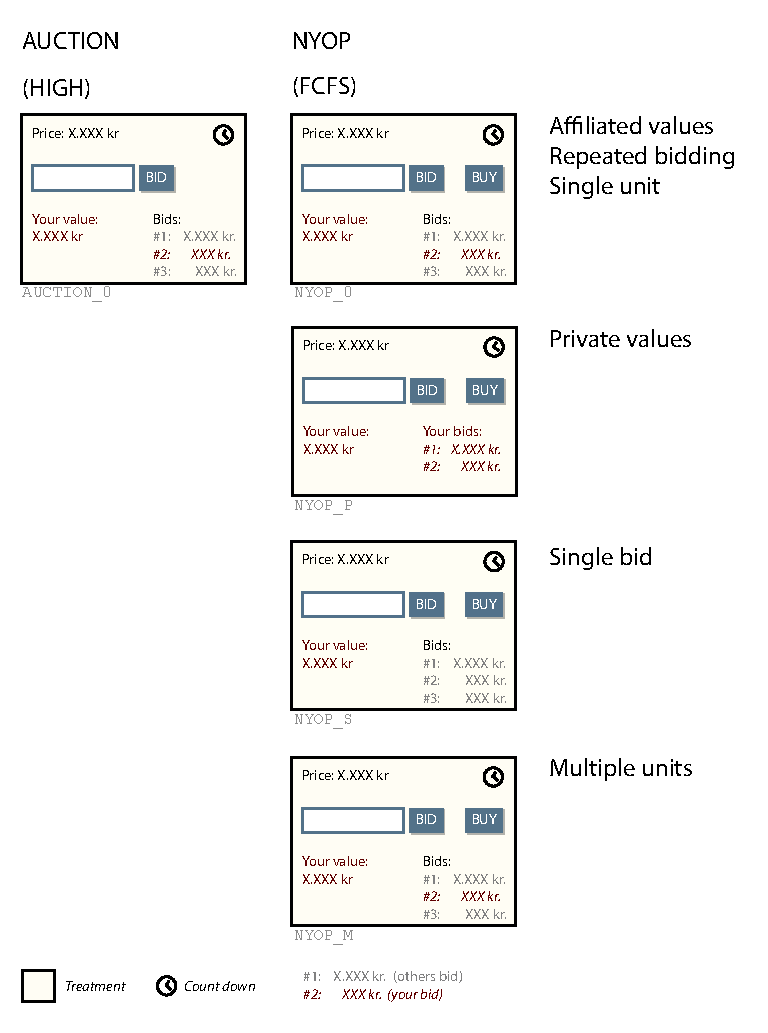
\includegraphics[width=\textwidth]{Figures/Treatments}
			\label{fig:treatments}
	\end{figure}

	There are five treatments see figure~\ref{fig:treatments}. The $NYOP_0$ treatment is the control. The two main treatments are; english auction ($AUCTION_0$) and NYOP ($NYOP_0$).
	In both buyers can repeatedly submit bids (repeated bidding). In the auction buyers can submit a higher bid out-bidding others or themselves. The auctions ends when the clock runs out, and the winner is the highest bidder. In the NYOP a buyer can `buy' or submit a bid, if the bid is above the threshold level, the buyer wins the object and the auction ends. If the bid is rejected, the buyer can `buy' or resubmit a new higher bid. This is the individual channel in which learning can happen. The NYOP ends once a buyer uses the `buy' option or once the seller receives a bid above the sellers threshold level. If no one buys and no bids submitted then the NYOP ends when the clock runs out.

	In both treatments all previously submitted bids are visible to all (affiliated values). Buyers can use this information to form and update expectations about the value of other buyers and about the seller's threshold level (in NYOP). This is the common channel through which learning can happen. Once the object is sold and the round ends, the posted price along with the winning bid is displayed to all buyers, before the next round initiates. This is done to avoid any confusion about the final selling price, since our interest is learning and how buyers form expectations about the threshold level. Displaying this information hopefully helps us minimise the effects of expectation errors.

	In both treatments a single unique unit is put up for sale (single unit). This together with the respective allocation rule introduces competition into both treatments. A comparison of these two treatments determines which mechanism gives the highest revenue. It is also possible to evaluate the efficiency of the two mechanisms\footnote{\label{footnote:efficient}An efficient allocation is when the object is allocated to the buyer will the highest value. This is an important consideration (for instance in government held auctions) where the seller also considers the subsequent surpluses. This could either be the winning bidder's surplus or customers of the winning bidder. This article is more aimed at art or antiques, were efficiency concerns are secondary to revenue concerns.}. However this seems unproductive as the NYOP would most likely be inefficient. Efficiency in the NYOP requires that the buyer with the highest value is fastest to evaluate the posted price, form expectations and the fastest to submit a bid above the threshold level. The FCFS allocation rule in NYOP does not promote efficiency. 

	The three additional NYOP treatments, trying to disentangle the counteracting effects of learning and competition, are:

	{\bf Multiple unit treatment} ($NYOP_M$). 
	By selling multiple units rather than a single unit the competition among buyers is reduced, while the learning and price discovery mechanism is unaffected. Winning bids are only displayed after the round ends, while bids below the threshold level are still shown to all. Buyers are not told how many unsold items remain only the total number of units for sale. When the round ends the posted price and all winning bids are shown. The number of units to sell in this treatment is somewhat arbitrary (see figure~\ref{fig:competition-items}). A non-arbitrary choice is the same number or more units than there are buyers (excess supply), as this completely eliminates competition. Minimum competition is as attended by selling $N-1$ units, and maximum by selling 1 unit. The multiple object treatment will sell $ceil(N/2)=3$ units. Competition changes in the multi object unit treatment, while learning is unaffected. Compared to $NYOP_0$ changes in revenue will be due to decreased competition among buyers.
	
	\begin{figure}[h]
	        \centering
	        \caption{Competition and number of items for sale}
	        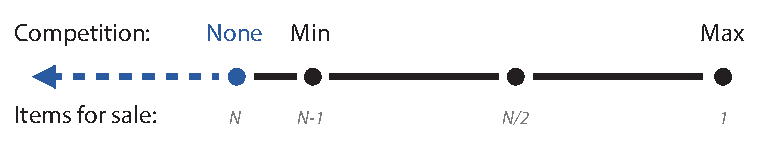
\includegraphics[width=0.7\textwidth]{Figures/Competition-Items}
			\label{fig:competition-items}
	\end{figure}

	{\bf Single bid treatment} ($NYOP_S$).
	In this treatment buyers are only allowed to submit one bid. If the bid is rejected they cannot resubmit a new nor buy. This restriction removes the buyer's ability to learn the threshold level through the individual channel (i.e. by repeatedly submitting incrementally increasing bids until the threshold level is reached). It is still possible to learn through the common channel. That is, buyers can still discover the threshold level, but it requires waiting for other buyers to submit their bids, and while waiting they risk that others win the object. The number of buyers might be crucially here, since faced with more competing buyers, one will be more hesitant to wait. Competition among buyers is not affected in the single bid treatment. Changes in revenue will be due to decreased price discovery, e.g. no learning takes place through the individual channel.

	{\bf Private value treatment} ($NYOP_P$).
	Another way in which price discovery will change is by restricting the common channel. This the the purpose of the private value treatment. Here buyers can only see their own bids. Buyers still have the ability to learn the threshold level though the individual channel, but they now have less information about competing buyers. Comparing the results from this treatment with the previous and $NYOP_0$ might help to answer how buyers discover the threshold level. Whether its by individually and repeatedly submitting bids or mainly through observing what others bid. When this treatment removes the option to observe others, do buyers then submit more individual bids? And are they further from guessing the true threshold level? And ultimately what are the effects on revenue? 

	\subsection{Participants: sample size, motivation and incentive problems.}


	\subsection{Technology and execution}
	The experiment will be built as a web-application. It will rely on Mozilla Labs' TogetherJS to enable simultaneous action of participants. Instead of using pre-build experimental software such as ztree, but by building the experiment as a web-application it becomes independent of platform (and can run on PC, Mac, Smartphone, Tablet, etc). And thus the experiment is not strictly restricted to a `lab' setting, but can easily be executed in classrooms, cafeterias, as well as over the internet. After running the experiment in the computer lab at University of Copenhagen with students of economics, the experiment can be run with other types of participants. But instead of inviting professionals or students with other majors into the lab, I can take the experiment to them. Participants are paid in cash, or using a micropayment service (MobilePay, Paypal, etc). I would like to run the experiment three times; inside the lab, in-person outside the lab, online.


	\subsection{Evaluating experiment -- interpreting results}
	
	\section{Conclusion}
	
			
	\newpage
	
%\renewcommand{\bibname}{Referencer}
\bibliographystyle{apalike-url}
\bibliography{ref}
	\nocite{*}
%	\begingroup
%		\renewcommand{\section}[2]{}%
%		\raggedright
%		\begin{thebibliography}{10}    
%
%
%		\end{thebibliography}
%	\endgroup


\end{document}